\section{Phase I Work and Feasibility Study}

The result of the Phase I project is a prototype of the VnV framework. As we will show,
this framework provides all the core functionality required to facilitate in-situ \VV and automated 
documentation generation in numerical simulations. 

The requirements set by the project team for the Phase I prototype were:

\begin{itemize}
 \item Cross library support. Most modern numerical simulations rely on a deep hierarchy of numerical simulation tools. For example, BISON, the fuel performance code in the NEAMS toolkit, is built using MOOSE; MOOSE uses libMesh; libMesh uses PETSc; PETSc uses hypre; and hypre uses BLAS. Thus, it is a requirement of the prototype that the system should provide a single interface for in-situ testing in any library linked to the final executable. 
 \item Multilingual support: The big three computing languages in high performance computing are C, C++ and FORTRAN. To ensure the system has wide applicability, it is essential that users be able to use the framework in software written in any one of these languages. 
 \item Run time configuration: Users should be able run \VV tests without needing to recompile either the executable or any of the linked libraries. The tests themselves should be completely independent from the source code and configurable at runtime. 
 \item Simple integration: The injection point system should be simple to integrate into existing applications.
 \item The framework should automatically generate a highly customizable, publication grade \VV report for each simulation. 
\end{itemize}

These requirements were chosen because they represent the core functionality required to facilitate the development of explainable numerical simulations. That is to say, in demonstrating this functionality, the project team will be able to prove the feasibility of the proposed approach in equipping general purpose numerical simulation toolkits with built in support for end-user solution verification and validation. 
\begin{figure}
\centering
 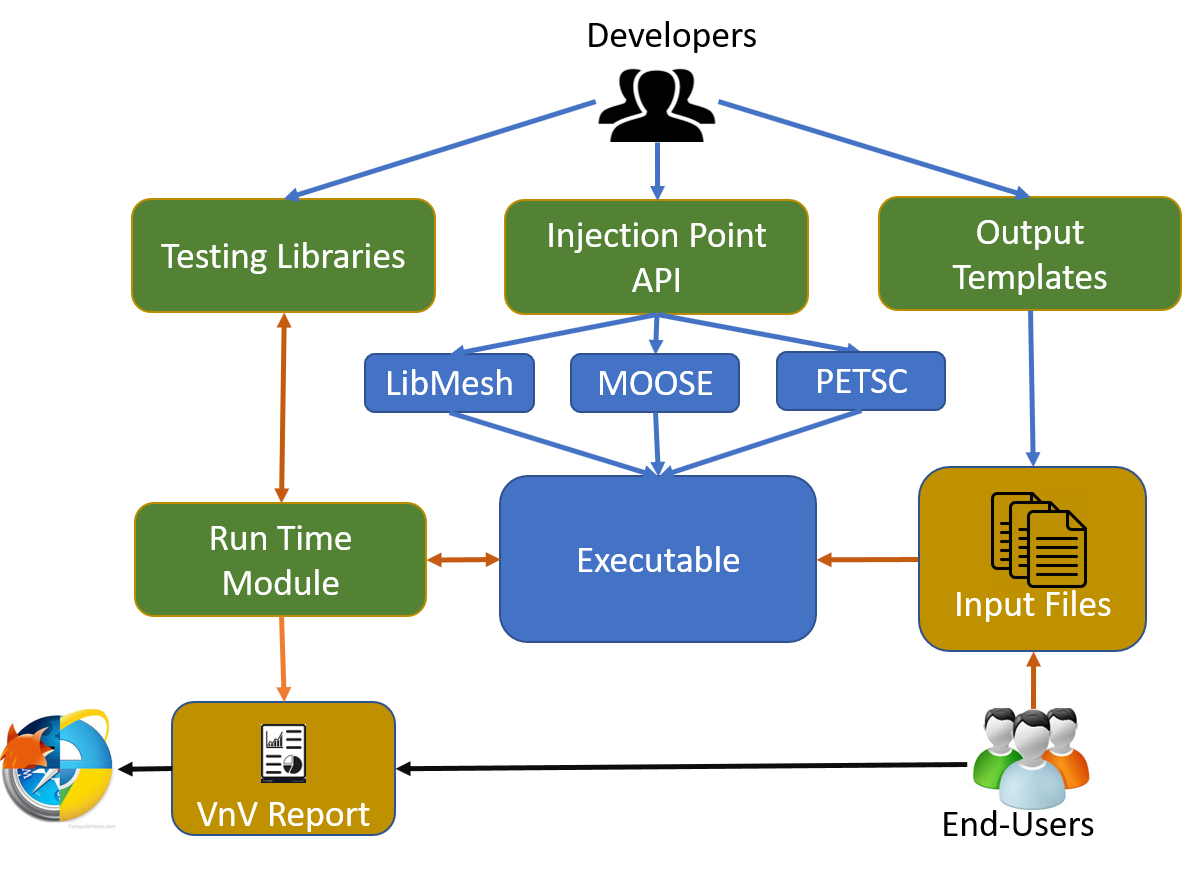
\includegraphics[width=0.7\textwidth]{./Figures/VnVOut.png}
 \caption{ The VnV toolkit development lifecycle. Here, green boxes represent core VnV functionalities. Developer interactions are shown in blue, runtime interactions are shown in orange and post-processing interactions are shown in black. \label{fig:toolchain} } 
\end{figure}
 
Figure~\ref{fig:toolchain} provides an example of how developers and end-users will interact with the VnV toolkit. In this case, we show an example of how the toolkit functionality might be implemented in the MOOSE toolchain. The first step in the VnV development life-cycle is to specify and describe the injection points. These injection points will be placed at key locations of the code where testing can and should take place. In the Phase II product, inserting an injection point into a code will be as simple as annotating some variables for inspection and calling an injection point function. In addition to adding the code, developers will also complete an output template that will be used in the final \VV reports to describe the state of the simulation each time that injection point is met. The VnV tests are developed in external libraries and hence, can be developed either by the developer of the simulation or by the end-user of the code. The core framework will also include a robust set of general purpose \VV tests. We envision that the developers of a numerical simulation package will ship the library with hard-coded injection points, a set of custom \VV tests and a number of VnV configuration files. 


\subsection{Task 1: Develop Routines for Data Collection with ADIOS. }

Work on task one began with a through investigation into the optimal approach for allowing injection points to be inserted 
into existing code bases. The goal of the task was to provide a simple mechanism for facilitating data collection and testing that required minimal changes to the build system, had small
overheads when testing was turned off, and that which could be removed from the final executable during compilation if need be. The project team investigated several approaches to doing this including
the development of a custom C pre-processor and an investigation into binary instrumentation with the Dyninst API.

In the end, it was decided that the best approach for performing \VV data collection and testing inside existing simulations was to produce a framework that allowed the
developer to hard-code injection points into the original source code. This approach is maintainable (the injection point specifications exist in the code-base), portable (it uses only
standard C functions) and efficient (pointers are used to avoid copying the data). In what follows, we describe the framework developed to support data collection and \VV testing 
in existing simulations. 

\subsubsection{Injection Points}

At the core of the framework are injection points. Injection points represent locations in a code where \VV testing can take place. Inserting an injection point into an existing function is a simple, three step process; (1) include the ``vv-runtime.h'' header file, (2) place injection points in the code and (3) write the injection point specification.

Declaring an injection point is as simple as calling the INJECTION\_POINT macro. The format for this macro is:

\begin{verbatim} 
INJECTION_POINT(<name>, <stage>, <type> <variable>,...)
\end{verbatim}

The macro is expanded to a variadic C function during preprocessing. Here, the unique name represents the id that will be used to define the injection point in the configuration files and the final reports. This name must be unique across all injection points in an executable. 

The stage parameter is an integer value that defines the step that this injection point belongs to. Using this parameter, the developer can set up multi-staged injection point testing. Tests defined on staged injection points stay in scope across all stages allowing tests to collect data across multiple code locations. The Phase I prototype supports up to 8000 stages at each injection point, although we have yet to come across a reason for an injection point with more than three or four stages. There are a few restrictions on the stage parameters to ensure efficient data output. First, a single stage injection point should be specified with a stage parameter of -1. A stage parameter less than 1000 should only be used to represent the starting point of a staged injection point. Likewise, a stage parameter greater than 9000 should be used to indicate that this is the last stage in the staged injection point. This allows a staged injection point to have multiple entry and exit points, while also allowing us to automatically handle recursion of injection points.  

The macro supports up to 25 separate variables; although we have not come across cases where more than 5 variables are required. Specifying a variable is as simple 
as writing its type and name. During preprocessing, the macro expands each variable-type declaration as 
\begin{verbatim}
 ..., <type> <name> , ... --> ..., "<type>", (void*) &name , ... 
\end{verbatim}

The runtime module of the framework then maps that void* pointer and the string based type specification to the user specified tests for processing. This is an obviously risky approach that, when implemented incorrectly, could lead to find memory corruption errors. For example, it would be easy for a developer to change the type of the variable in the code, but forget to update the string in the injection point declaration. A key goal of the Phase II work will be to develop a custom pragma directive that automatically detects the correct type for each variable. 

Figure~\ref{ip_example} shows a class for evaluating a linear function that has been enhanced with a single stage VnV injection point (the stage parameter is -1). 

\begin{figure}
 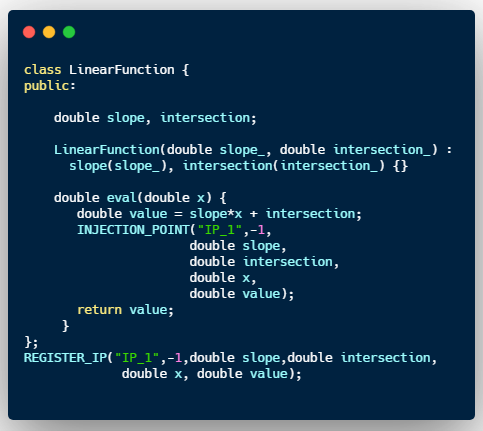
\includegraphics[width=\textwidth]{./Figures/linear-func.png}
 \caption{A code Snippet showing a member function enhanced with a single stage injection point called ``IP\_1``. This injection point is declared inside a member function 
 designed to evaluate a linear function at a particular value of $x$. This injection point provides access to the member variables describing the slope and intersection point
 of the linear function, the input parameter $x$ that defines where the function should be evaluated and to the result that will be returned. A user could add a simple test to 
 verify the accuracy of the value being returned and/or to assert that the slope and intersection are correct in accordance with the physical model they are attempting to simulate. 
 \label{ip_example}}
\end{figure}

In C++ codes, the developer can also opt to pre-register the injection point with the runtime module using the REGISTER\_IP macro. The macro uses a feature of object orientated programming languages that allows code in the constructors of static variables to be executed prior to the main function. In this way, one can register certain code elements by simply defining a static variable. Self registration is particularly nice because it allows for run-time detection of the injection points present in the call-graph. That information allows for the automatic generation of a customized test configuration file for each executable. All calls to the REGISTER\_IP macro should be made outside of function calls and classes, as shown in the last line of the code snippet in Figure~\ref{ip_example}. Unfortunately, static variables can only be initialized with constant expressions known at compile time in C and FORTRAN, so instead, information about injection points must be determined either by running the full simulation, or by pulling information from the injection point specification files. The custom compiler extension developed in Phase II will address this issue by hardwiring information about the included injection points into the meta-data of the executable or library. 

\subsubsection{The Testing Interface} 

The second facet of the framework is the \VV testing interface. The development of the 
test interface was based on the idea that tests should be loaded at runtime and defined independently of the source code. To achieve this, the test
interface was built using an C++ plugin pattern. This pattern allows users to develop tests in separate testing modules that can be loaded and configured 
at runtime using an XML configuration file. This allows the users to add or remove tests from injection points located in any linked library without ever 
needing to recompile the executable or any of the libraries. 

The first step in the development of a new VnV test is to create a testing library. The framework includes a library generation script that will automatically build the directory structure and makefiles required to 
build this library. Once the library has been initialized, the user can begin to develop individual tests. 


\begin{figure}
 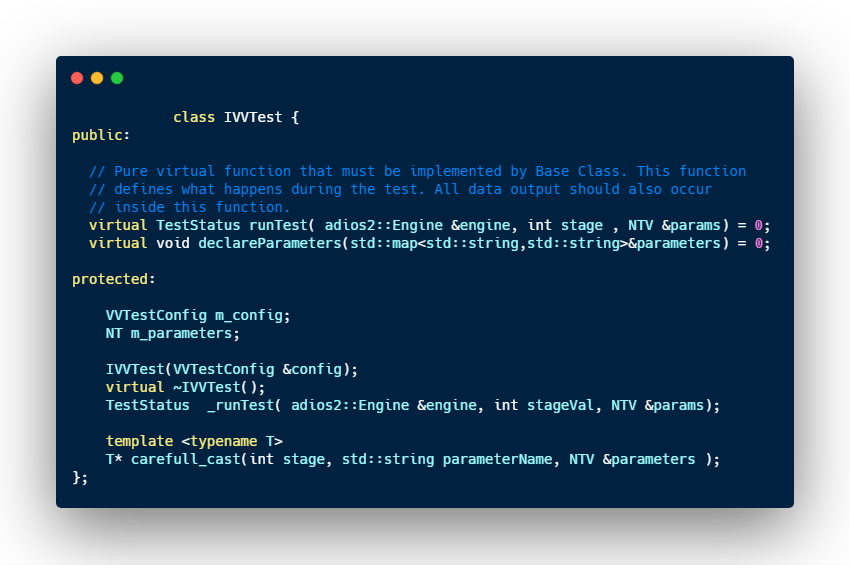
\includegraphics[width=\textwidth]{./Figures/test-interface.png}
 \caption{The IVVTest Interface. The framework includes a test generation script that generates all the boiler plate code required to implement this interface. All the developer
 needs to do is implement the ''declareParameters`` function and the ''runTests`` function. \label{test-inter}} 
\end{figure}



Figure~\ref{test-inter} shows the declaration for the IVVTest interface that needs to be implemented when developing a new test. To simplify the process of writing tests, the VnV framework includes a test generation this script. If the library generation script was used, this script will be available in the src directory of the new testing library. To run this script, the user should provide a unique name for the test and a list of the names and types of parameters that will be supported by the new Test. Using this information, the script generates all the boiler plate code required to implement the IVVTest interface and to handle all the required type-casting. 


\begin{figure}
 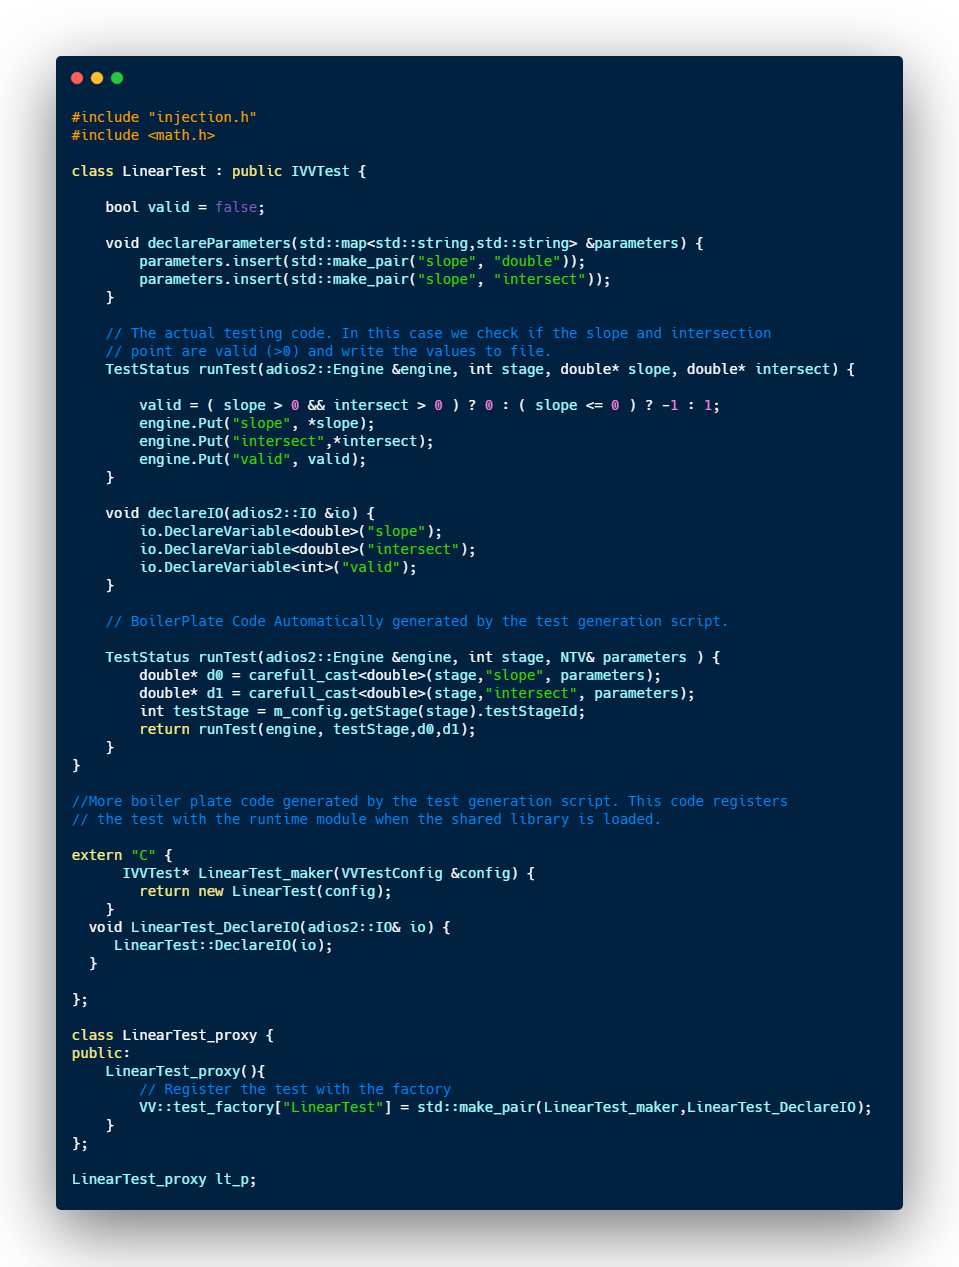
\includegraphics[height=0.9\textheight, width=\textwidth]{./Figures/test-examp.png}
 \caption{An example of a custom VnV test. In this case we implement a test that checks that the slope and intersection point of the linear function are positive and writes
 the result to file. \label{test-examp}}
\end{figure}


Implementing the interface is a three step process. First, the developer should implement the delcareParameters function. In this function, the developer will
list the parameter names and types that will be supported by the test. For example, the test shown in Figure~\ref{test-examp} supports the declaration of 
two parameters, a double named slope and a double named intercept. The user will map the injection point parameters to the test parameters at runtime using 
the test configuration file.

The main function of the test is the ''runTests`` function. The test generation script does all the dirty work required to cast the injection point parameters
to their correct object types. As shown in Figure~\ref{test-examp}, the user is then required to implement a single function of the form
\begin{verbatim}
 TestStatus runTests(adios2::Engine &engine, int testStage, ...);
\end{verbatim}

Here, testStage is an integer representing the stage that the test is currently in. A test can support as many stages as there are integers. As will be shown below, the test 
stages are mapped to injection point stages at runtime using the test configuration file. The ... represents pointers to the variables requested by the test in the 
declareParameters function. 

Data output can occur at any point in the runTests functions. The core runtime module ensures that each test stage is completed in a unique ADIOS2 step. This allows for efficient 
compartmentalization of the test output and makes post-processing significantly easier. Data output is completed directly in ADIOS through the 
ADIOS2 read/write API and the adios2::Engine. For example, the Test shown in Figure~\ref{test-examp} writes the slope and intersect points received from the injection point
to file along with an integer representing the validity of those values. 

The next step is to pre declare the IO variables that the test will utilize. This is optional, however, it is considered best practice because it allows for optimizations 
in the handling of the meta-data inside ADIOS. The final step in writing the test is to register the test. Registration provides the core runtime module with the information 
necessary to initialize the test at runtime. The test generation script automatically generates the code required to do this, 
hence, no further input is required from the develop on this part. 

\subsubsection{Variable Transform}

In addition to tests, the VnV framework also provides support for pluggable variable transforms that can be used to 
map injection point parameters into formats that can be consumed by the tests. These Test modifiers are developed using 
the same plugin based C++ pattern used to define the tests and can be included in seperate Modifier libraries or as seperate 
components in existing testing libraries. Some examples of modifiers implemented during the Phase I testing include; a dereference modifier
that dereferences a pointer variable; an array access modifier that pulls out the $n$'th element from an array variable. Figure~\ref{test-mod} shows
a modifier that extracts a PETSc PC object from a KSP object prior to testing. This allows the developer to call tests that work with the PC object from
injection points that only pass the KSP. 

\begin{figure}
 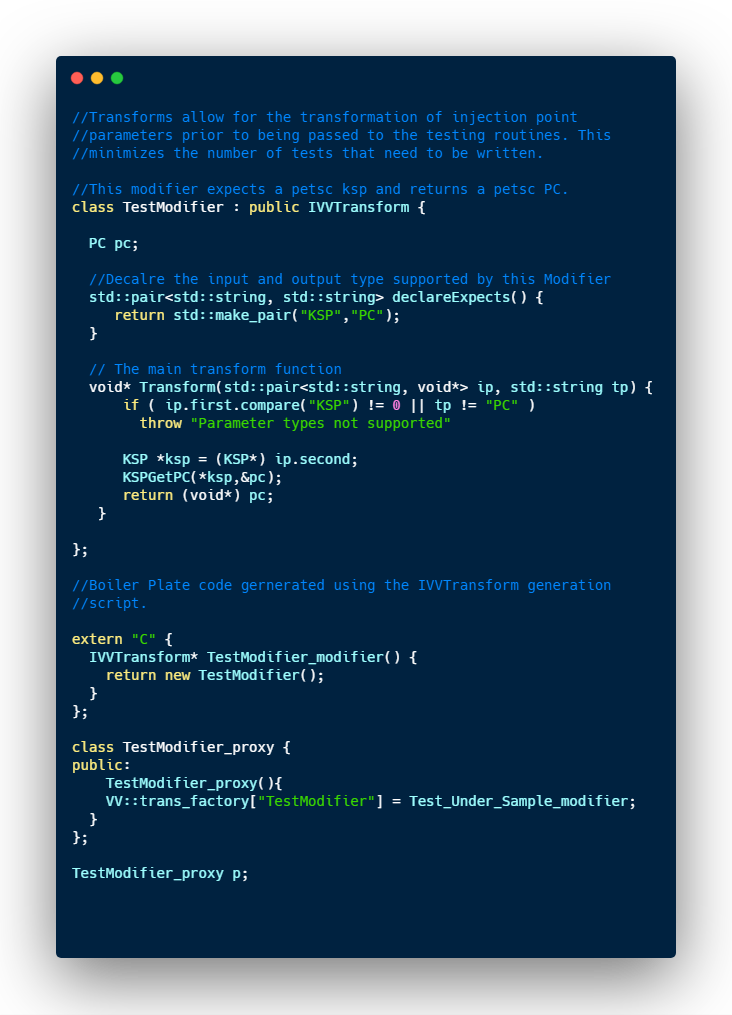
\includegraphics[height=0.9\textheight, width=\textwidth]{./Figures/test-modifier.png}
 \caption{An example of a custom VnV test. In this case we implement a test that checks that the slope and intersection point of the linear function are positive and writes
 the result to file. \label{test-mod}}
\end{figure}


\subsubsection{The VnV Runtime Module}

The VnV runtime module is the driving force behind the framework. This module contains all the functionality required to detect the injection points, parse the
configuration file, setup the ADIOS IO engine, load the external testing libraries and run all the tests.

Configuring a simulation to use the VnV framework is a simple, four step task; (1) include the header file, (2) Call the VVInit function at the start of main, (3) Call the VVFinalize function
before exiting, and (4) link the VnV library to the main library along with any required sub-libraries. 

The users primary interaction with the VnV runtime module is through the XML configuration file. The full XSD specification for the input 
files is shown in Figure~\ref{fig:xsd_specification}. 

\begin{figure}
\centering
 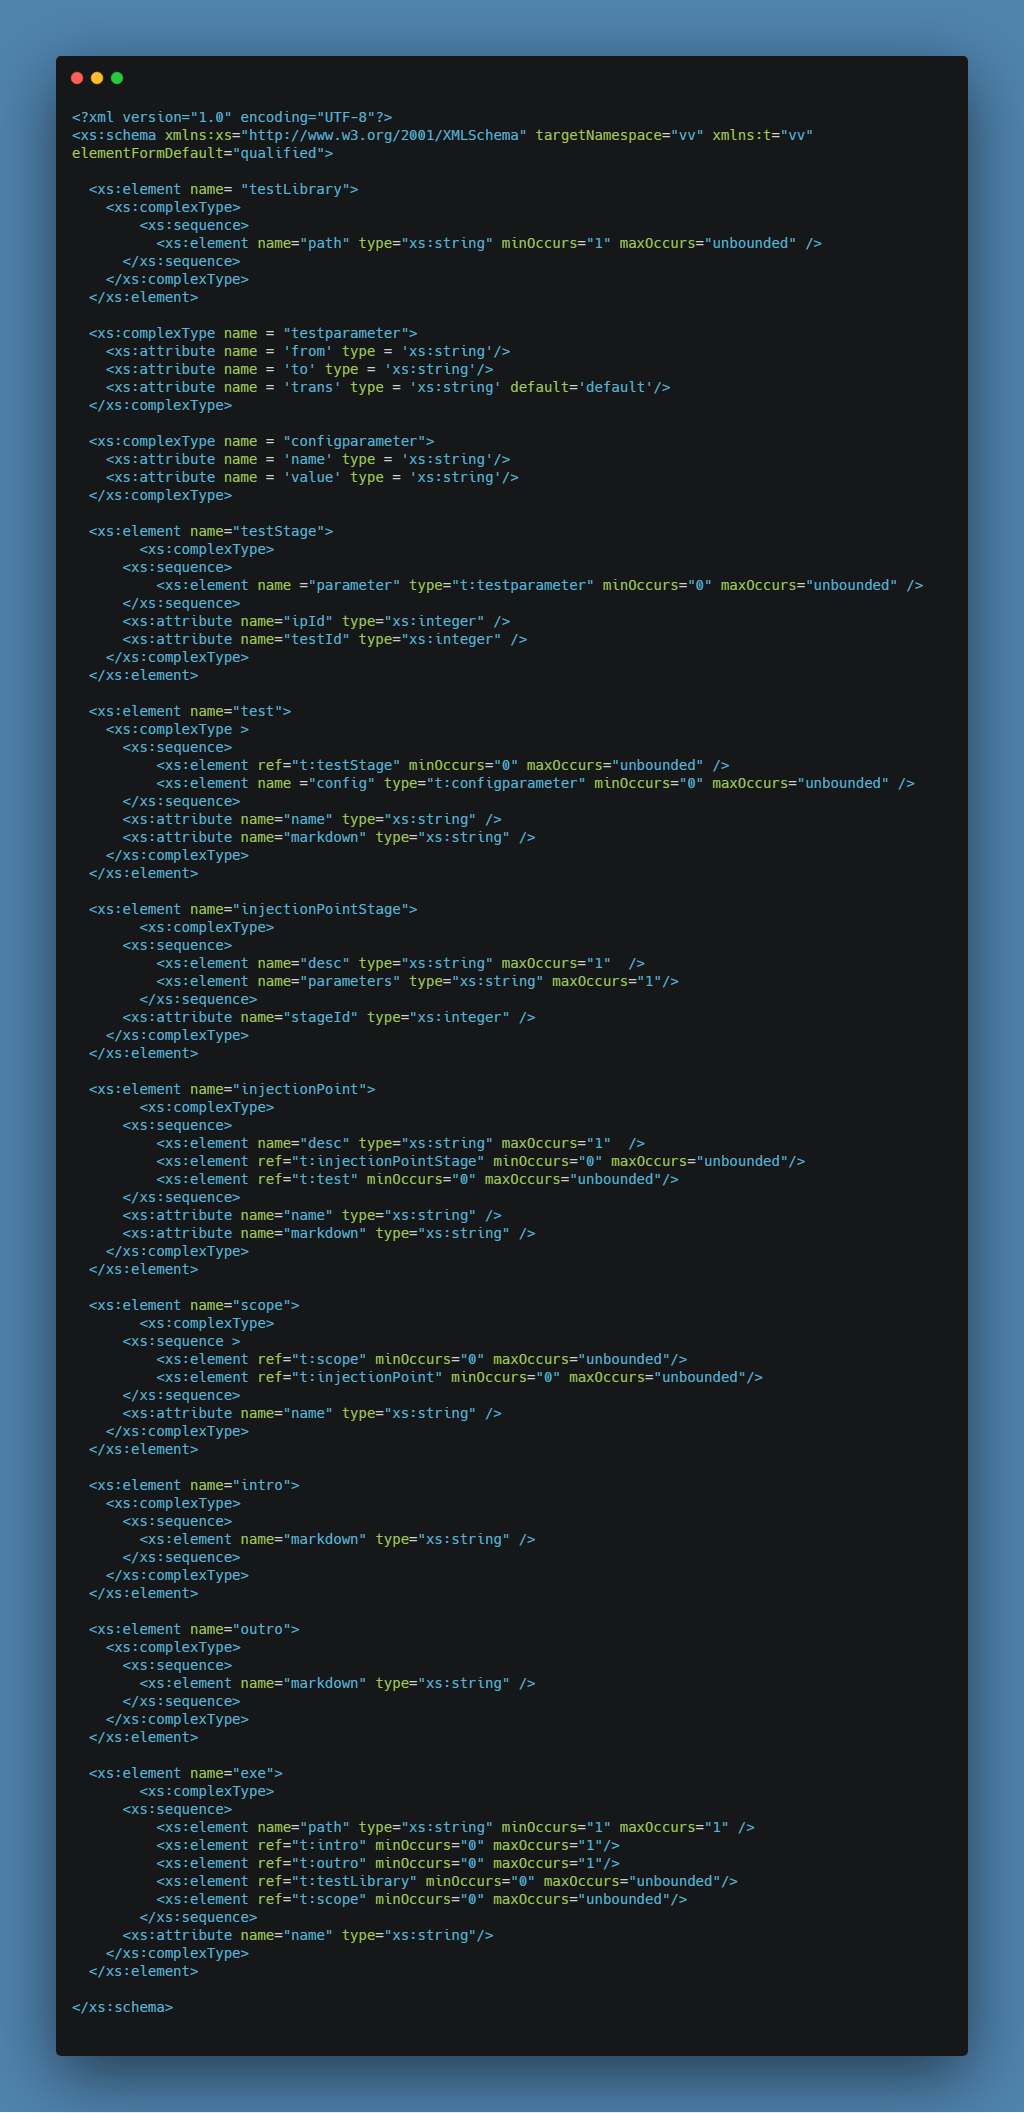
\includegraphics[height=0.9\textheight, width=\textwidth, keepaspectratio]{./Figures/xsd-schema.png}
\caption{The XSD specification for the input configuration file. The VnV framework uses this specification in conjunction with Xsd2Cpp to automatically generate
a fully featured XML Parsing library with support for reading, writing and validating XML files. \label{fig:xsd_specification}}
 \end{figure}

A full XML parser was built for the input file specification using XSD2Cpp. The parser allows for reading and writing input files based on the XSD specification and has built 
in support for input file validation. This makes it incredibly easy to parse and validate the XML input files. 

\begin{figure}
 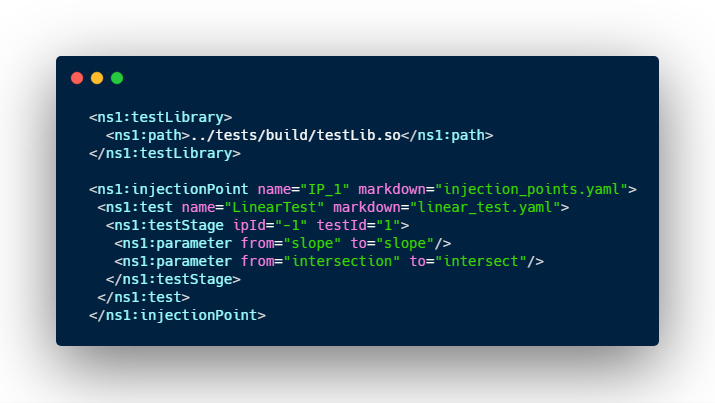
\includegraphics[width=\textwidth]{./Figures/test-xml1.png}
 \caption{An example of the XML configuration file for attaching test to injection points at runtime. In this case, we attach the LinearTest test shown in Figure~\ref{test-examp} to the ''IP\_1''
 injection point shown in Figure~\ref{ip_example}. \label{test-xml}}
\end{figure}

Figure~\ref{test-xml} shows a snippet of the XML file required to setup a test at an injection point. The first step to injecting a test
is to load the test library. This is as simple as specifying the path to the library in the ``testLibray'' element. This element supports
the specification of multiple paths, making it very easy to include multiple libraries. In this case, we include a test library located in
the tests directory called testLib.so.

The second step to injecting a test is to define the injection point. The Phase I prototype can automatically generate
an input file that contains all registered injection points; however, including a non-registered injection point is a simple 
task. The only required parameters for an injection point are the ``name'' and ``markdown'' attributes. The ``name'' attribute
represents the unique name given to the injection point in the code. The markdown attribute should be the path to a file that 
contains the YAML based specification for the injection point (described below).

To specify a test, the user must provide the unique name of the test and the path to the
YAML based specification file for the test. 

The testStage element allows the user to map the injection point stages to the test stages. This is completed using the ipId and
testId parameters. In Figure~\ref{test-xml}, we attach the LinearTest test shown in Figure~\ref{test-examp} to the single stage ''IP\_1''
 injection point shown in Figure~\ref{ip_example}. 

 
Once the input file has been created, turning on testing using the VnV framework is as simple as calling the Initialization function with the correct filename. Runtime 
validation of the input file is completed at this time. For registered injection points, this includes checks to ensure the parameter mapping specified in the input file
are valid. For un-registered injection points, this validation must be completed at runtime. In that case, if a parameter mapping is found to be invalid, the runtime module 
prints out an error and skips that test. 

\subsection{Task 2: Prototype Several VnV Tools } 

Using the framework defined above, the project team developed a small VnV testing library for inspecting the values of data stored in
C++ vectors. 

Figure~\ref{fig:euclid_test} shows an example of one of the tests supported in this prototype library. In this case the test calculates the euclidean
error between two C++ vectors. The output out the test is a double representing the error. 

\begin{figure}
 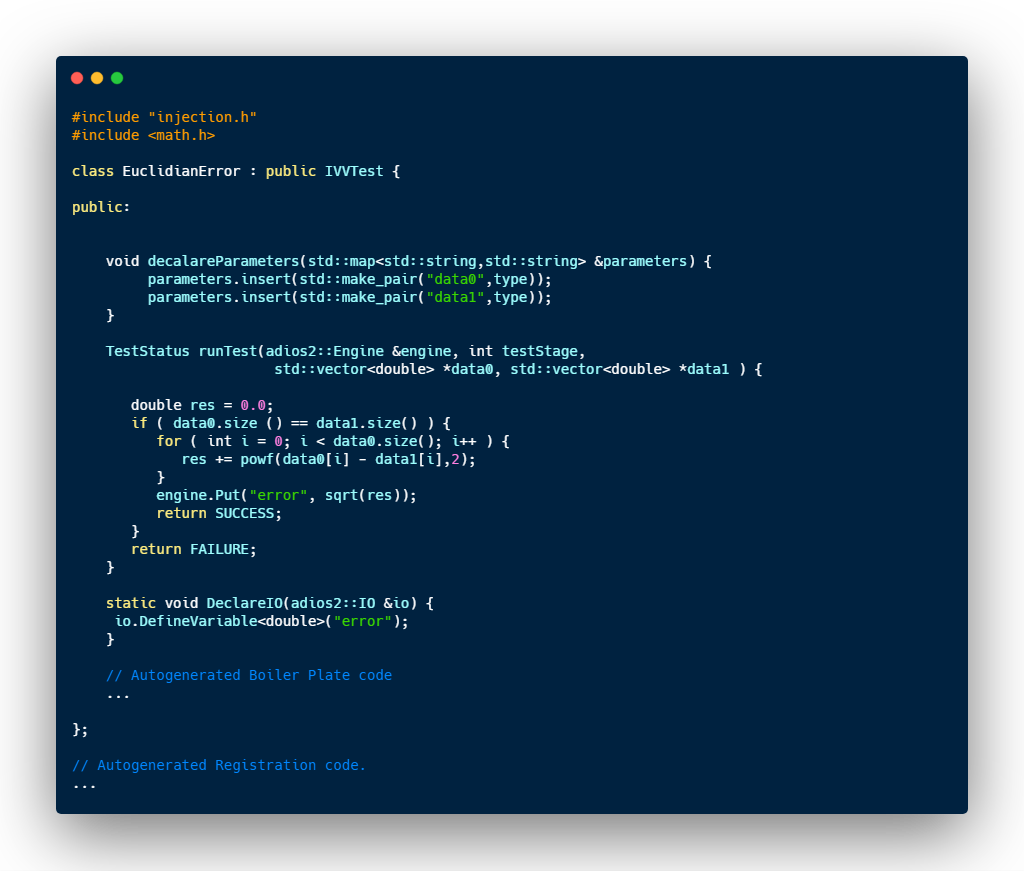
\includegraphics[width=\textwidth]{./Figures/euclid-test.png}
\caption{ The testing code for the beginnings of a VnV testing library for making statistical assertions regarding the data stored in distributed arrays. Amongst other things,
the Phase I prototype supports calculating the Euclidean error between two vectors. The Phase II effort will look to extend this support to include a range of efficient statistical
methods that can be applied to data stored in distributed arrays. \label{fig:euclid_test}}
 \end{figure}

Other tools included in the library include a tool for calculating vector norms, a tool for asserting that all values in the vector are positive, 
and a tool for plotting the vector on a line chart. A key goal of the Phase II project will be to extend this library to support evaluations on distributed arrays. Distributed arrays are particularly 
tricky because the testing algorithms will have no knowledge of how the data is distributed across the processors. 

\subsection{Task 3: Prototype the Graphical User Interface.} 

The final task of the Phase I project was to develop a GUI for the VnV toolkit. In particular, the Phase I effort focused on developing the software interfaces
required to visualize the data output during VnV testing. 

After accessing the strengths and weaknesses of multiple different approaches, the project team decided to develop the VnV data visualization interface using HTML and Javascript. The primary benefit of this approach is portability - the report can be displayed in any web browser - but other benefits include interactive components, non-linear data presentation and high levels of customization. Moreover, the server-less nature of the HTML web-page allows for direct publication on any static web hosting service (github.io, AWS S3, etc.). 

The goal of the Phase I project was to create an interface that allowed for automated, informative post-processing of the data output during VnV testing. To do this, the project team developed the VnV automated documentation generation system. 

This system is built around the fact that simulations are built up of a large number of smaller functions, each with a specific pre-defined task and an expected result. This compartmentalization makes it very easy to write generic templates that describe what is happening at each function and during each injection point. Likewise, while the inputs to VnV tests might change, the overall structure of the outputs is constant. For example, the LinearTest shown above always outputs the slope and intersection points to file. This makes it very easy to write template specifications that can be populated with data during post-processing the produce an informative, customized report. 

The VnV framework implements this functionality using a combination of the YAML file format and a custom markdown specification. Figure~\ref{fig:test-spec} gives an example of this YAML
markdown file that provides templates for the ``IP\_1'' injection point shown in Figure~\ref{ip_example} and for the LinearTest test in Figure~\ref{test-examp}. The fields supported in the YAML specification for each test and injection point are:

\begin{itemize}
 \item {\bf title:} A descriptive title for the injection point 
 \item {\bf content:} A markdown formatted string representing the content to be displayed for this injection point in the final report.
 \item {\bf sections:} A map containing the content for any subsections to be displayed under the original content description. Each subsection is displayed  as a collapsible child or its parents content panel and is included in the overall index of the final report. 
 \end{itemize}

During compilation, the automatic documentation generation script loops through every injection point recorded in the VnV output file. For each injection point, the script locates the injection point specification using the markdown attribute provided in the input configuration file, renders it in html, and adds it as a new section in the final report. Similarly, for each test, the script locates the test specification and renders it as as subsection in the injection point section. 

The defining feature of the specification files is the support for writing the content using a custom markdown format that provides support for automating data post-processing and visualization. In particular, this custom markdown format is designed to facilitate direct interaction with the data collected during the VnV testing Phase. In this way, users can write generic markdown specifications that are automatically populated with data during rendering.   

The Extended markdown format for numerical simulations, MD-XNS,  was developed for the VnV project as a highly customizable system for automatically processing the results obtained from numerical simulations into interactive, informative HTML/JS web pages. The extension itself was built using py-markdown, an open source python library for converting markdown files into html. In addition to standard markdown commands, the MD-XNS format supports custom post-processing commands of the form 

\begin{verbatim}
[VV::<name>={...},...], 
\end{verbatim}
where name is the name of the component the user would like to insert and {...} represents a dictionary of configuration options. The key feature of the MD-XNS format is that it supports direct interaction with data stored at each ADIOS step. In the markdown specification, this data is accessed through the following syntax: 
\begin{verbatim}
 [DATA::<name>={...}] 
\end{verbatim}
Here, the name represents the name of the data element to be inserted. The following library allows for specific type formating information, although that support has not been implemented in the Phase I prototype yet. The data that is available in a markdown specification depends on the injection point and test that the specification was written for. For example, the slope, intersect and valid parameters written by the LinearTest test could be queried when writing the test specification for the LinearTest test. In this way, developers of tests can write simple markdown specifications that render into highly informative, interactive data visualizations without ever having to process the data. This allows for the creation of living, breathing VnV reports that evolve as the simulation is developed. Figure~\ref{fig:test-spec} shows an example test specification for the ``IP\_1'' injection point and the LinearTest test. 

\begin{figure}
 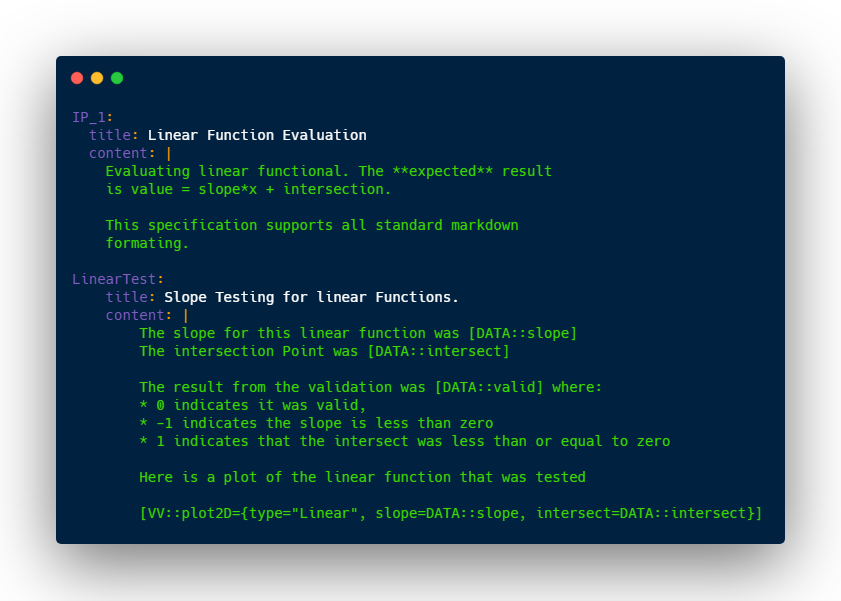
\includegraphics[width=\textwidth]{./Figures/yaml-md.png}
\caption{ An example YAML specification file. In this case, the test LinearTest uses the DATA API to extract the values for the slope and intersect provided by the injection 
point. The test specification then uses the support for two dimensional plotting to generate a linear plot with the appropriate slope and intersect point. \label{fig:test-spec}}
 \end{figure}

The Phase I prototype has limited support for a number of custom data visualization routines including 
\begin{itemize}
\item Table: The table command inserts an interactive, sortable, search-able table into the final HTML document. The user can populate the table by entering the information
manaully, by providing the name of a csv file, and/or by using data generated at runtime. 
\item Chart2D: The Chart2D command inserts an interactive Charts.JS chart into the document. The entire array of Charts.JS charts are available through this component, including bar, 
line, scatter and pie charts. In each case, the chart is configured using a python dictionary entered directly into the markdown. 
\item VTPView: The VTPView command uses VTK.js to insert interactive 3D visualization of a .VTP files in the final document. 
\item PostPro: The PostPro function allows the user to set up post-processing scripts for execution during the report generation phase. In this way,
users can write simple scripts that parse the data into formats more suitable for use in any of the other data visualization components. 
\item ThreeJs: The ThreeJS command provides another approach for integrating three dimensional visualization in the final report, in this case using three.js for rendering. This 
component is particularly useful for viewing meshes. 
\end{itemize}

Figure~\ref{rendered-example} shows a screenshot of a VnV report generated using this approach. The main layout consists of two components; the index and the content. The index in generated directly from the VnV output file. Each entry in the index represents an injection point that was reached during the execution of the simulation. If a new injection point was reached during the first and last steps of another staged injection point, that injection point is listed as a child node in the index. In this way, the index represents a coarse grained view of the simulations call stack, whereby the injection points represent the nodes. The content section is generated automatically from the YAML specification files. In this case, the user has completed a test titled ``Linear Function Plotter'' inside an injection point called ``Linear Function Constructor''. 

\begin{figure}
 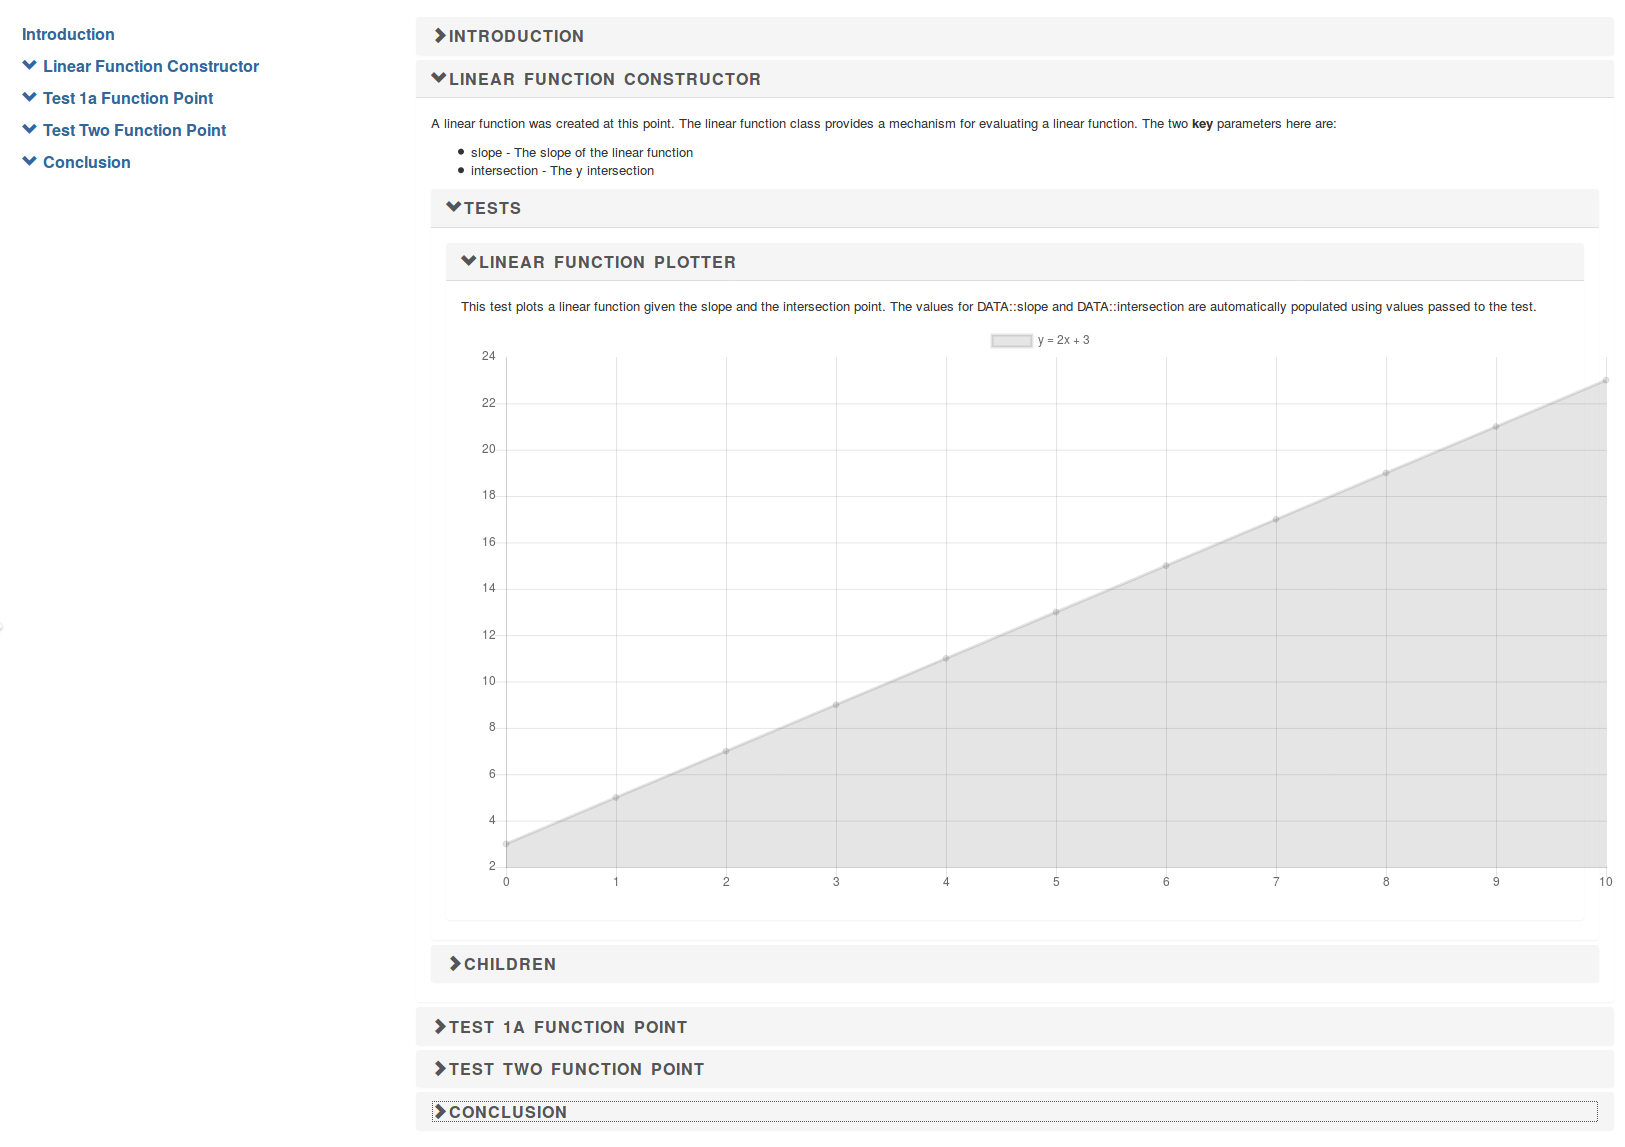
\includegraphics[width=\textwidth]{./Figures/render-example.PNG}
\caption{ An example of the VnV report generated automatically from the VnV output files and the injection point and test specification files. \label{rendered-example}}
 \end{figure}


The key point to note here is that this interface was generated automatically from the VnV output file. Once the test and injection point specifications have been written, no user action 
is required to build this fully interactive VnV report. As stated earlier, we envision that developers of simulation libraries (e.g., PETSc, libMesh, hypre) would ship their codes with the injection 
points hard coded into the source code along with any custom VnV testing libraries. Those developers would also provide their users with the injection point specification files, the test specification
files, and the input configuration files required to support end-user \VV for there library.

Using these files, the end-users of those packages, i.e., the developers of actual numerical simulations, can then form a single input file that configures \VV testing in every VnV equipt
library linked to the final executable. In this way, the \VV toolkit provides a mechanism for generating explainable numerical simulations that not only provide the solution, but also a
detailed report on how the solution was obtained and why it can be trusted.

The Phase I proposal had initially stated that the Phase I GUI prototype would include support for setting up input files. However, after developing the framework, and using the input specifications, it became clear that a ``click'' style user interface would not be all that useful for setting up the configuration files. Rather, text-editor with context aware auto-completions and validations as is present in the NEAMS workbench is likely the best option.  As discussed above, the project team developed a XSD specification for the input file format. This specification contains the majority of the information required to setup context aware auto complete when building the input file. However, due to the evolving nature of the inputs; and with the further changes likely to occur in the Phase II project, it would have been highly inefficient to develop the input file GUI support in Phase I. As such, the development of a GUI for editing input files was delayed until Phase II. 

The VnV report generation system was written using HTML and JS to ensure portability and applicability for a wide range of users. However, this does not limit, in any way, the ability to view the VnV reports inside the NEAMS workbench. To prove this fact, the project team created a QT application that uses the QWebEngineView to display the HTML VnV report. This QWebEngineView allows for direct interaction with the report in any QT application. In Phase II, the project team will look to improve on this integration by allowing for input files to be specified directly in the MOOSE input files using the NEAMS support for context aware auto-complete and input validation. 

